%TODO : Beschreibung
Datensatz: glass

Die Fl\"ache unter ROC:

\begin{tabular}{c|c|c|c}
				Regellerner       & \emph{build wind float} & \emph{containers} & \emph{tableware}  \\ \hline
				\emph{J48}			& 0.81 & 0.87 & 0.93  \\ \hline
				\emph{Naive Bayes}  & 0.71 & 0.84 & 0.98  
\end{tabular}
\begin{figure}[htbp]
	\centering
		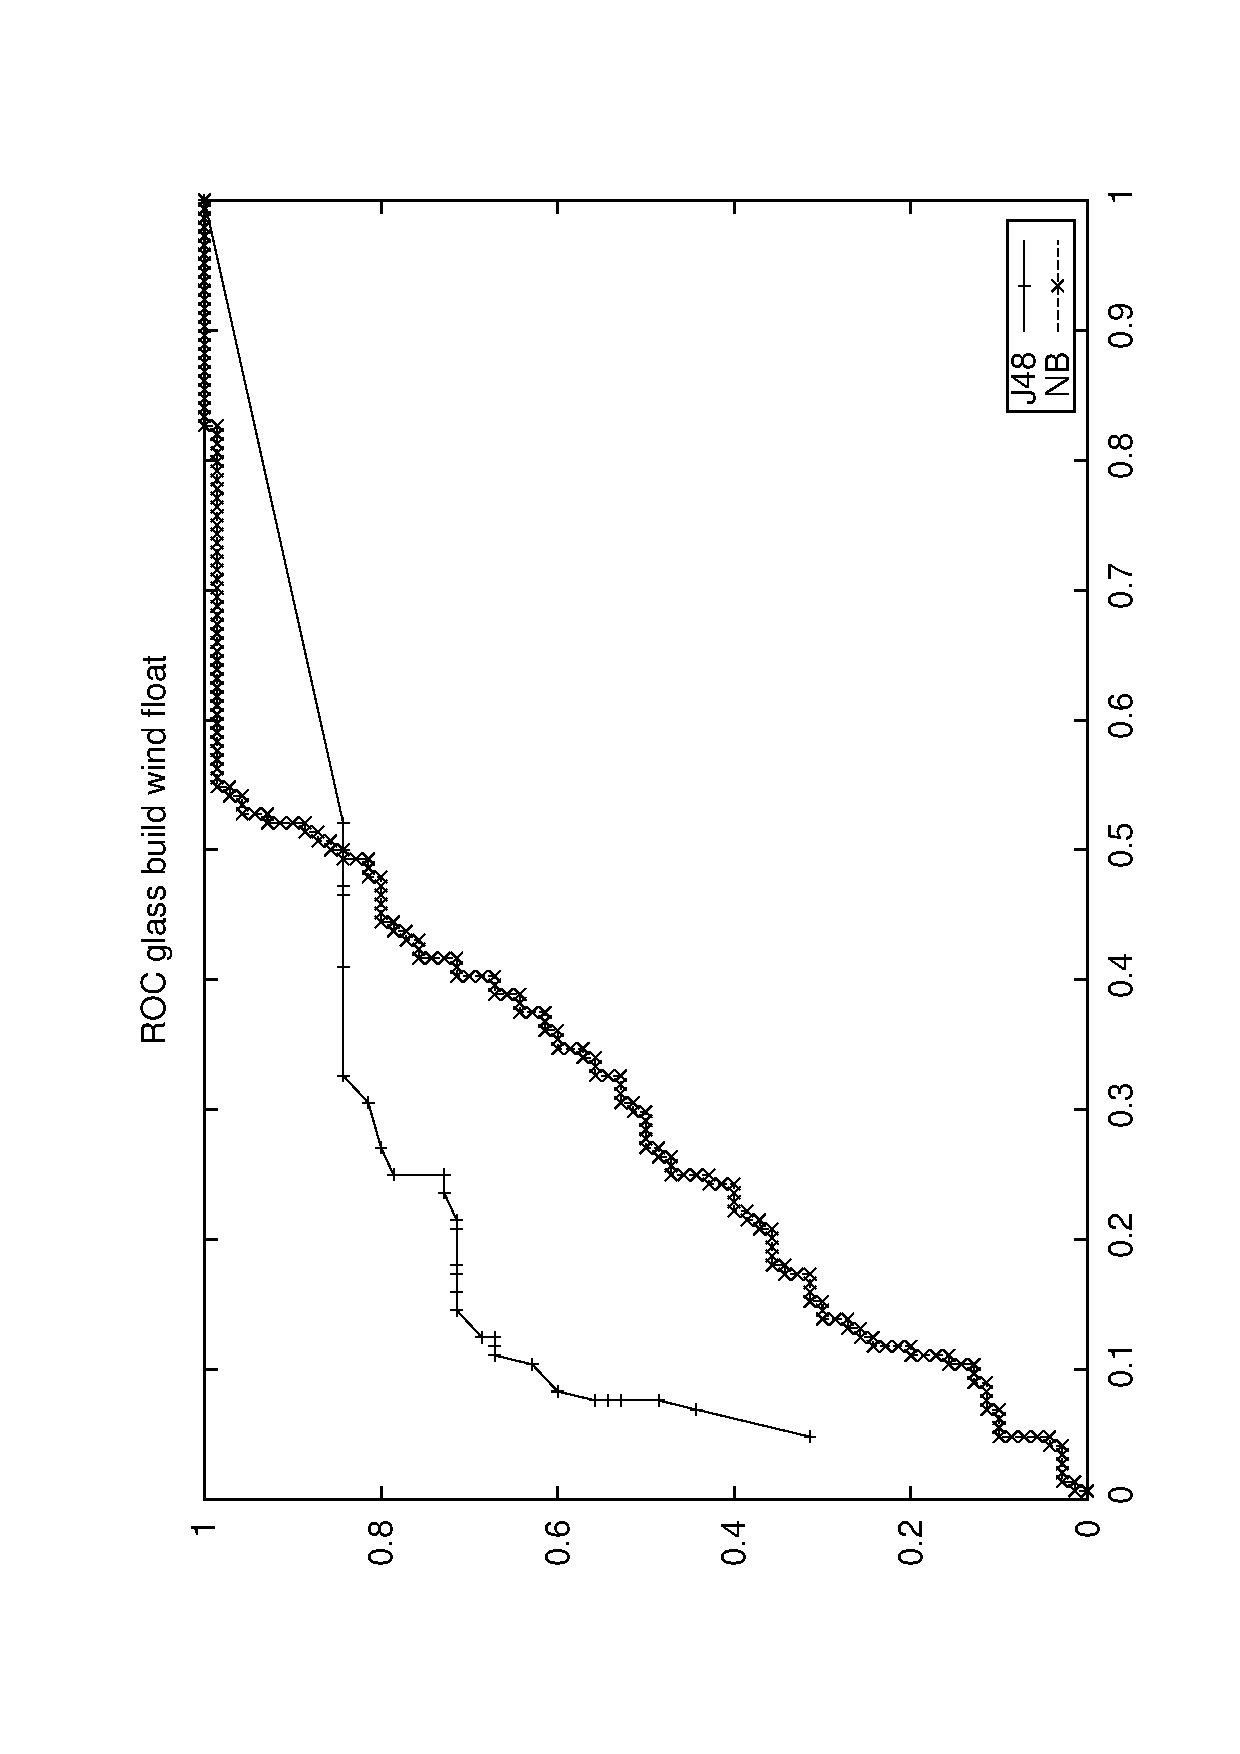
\includegraphics[height=3in]{pics/a3/ROC_glass_build_wind_float.pdf}
	\caption{caption}
	\label{fig:pics_a3_ROC_glass_build_wind_float}
\end{figure}

\begin{figure}[htbp]
	\centering
		\includegraphics[height=3in]{pics/a3/ROC_glass_containers.pdf}
	\caption{caption}
	\label{fig:pics_a3_ROC_glass_containers}
\end{figure}

\begin{figure}[htbp]
	\centering
		\includegraphics[height=3in]{pics/a3/ROC_glass_tableware.pdf}
	\caption{caption}
	\label{fig:pics_a3_ROC_glass_tableware}
\end{figure}


Datensatz: iris

Die Fläche unter ROC:


\begin{tabular}{c|c|c}
				Regellerner       & \emph{versicolor} & \emph{virginica}  \\ \hline
				\emph{J48}			& 0.952 & 0.961  \\ \hline
				\emph{Naive Bayes}  & 0.992 & 0.992  
\end{tabular}

\begin{figure}[htbp]
	\centering
		\includegraphics[height=3in]{pics/a3/ROC_iris_versi.pdf}
	\caption{caption}
	\label{fig:pics_a3_ROC_iris_versi}
\end{figure}


\begin{figure}[htbp]
	\centering
		\includegraphics[height=3in]{pics/a3/ROC_iris_virgi.pdf}
	\caption{caption}
	\label{fig:pics_a3_ROC_iris_virgi}
\end{figure}

